\documentclass[12pt]{article}
%%---------------------------------------------------------------------
% packages
% geometry
\usepackage{geometry}
% font
\usepackage{fontspec}
\defaultfontfeatures{Mapping=tex-text}  %%如果没有它,会有一些 tex 特殊字符无法正常使用,比如连字符。
\usepackage{xunicode,xltxtra}
\usepackage[BoldFont,SlantFont,CJKnumber,CJKchecksingle]{xeCJK}  % \CJKnumber{12345}: 一万二千三百四十五
\usepackage{CJKfntef}  %%实现对汉字加点、下划线等。
\usepackage{pifont}  % \ding{}
% math
\usepackage{amsmath,amsfonts,amssymb}
% color
\usepackage{color}
\usepackage{xcolor}
\definecolor{EYE}{RGB}{199,237,204}
\definecolor{FLY}{RGB}{128,0,128}
\definecolor{ZHY}{RGB}{139,0,255}
% graphics
\usepackage[americaninductors,europeanresistors]{circuitikz}
\usepackage{tikz}
\usetikzlibrary{positioning,arrows,shadows,shapes,calc,mindmap,trees,backgrounds}  % placements=positioning
\usepackage{graphicx}  % \includegraphics[]{}
\usepackage{subfigure}  %%图形或表格并排排列
% table
\usepackage{colortbl,dcolumn}  %% 彩色表格
\usepackage{multirow}
\usepackage{multicol}
\usepackage{booktabs}
% code
\usepackage{fancyvrb}
\usepackage{listings}
% title
\usepackage{titlesec}
% head/foot
\usepackage{fancyhdr}
% ref
\usepackage{hyperref} %生成可链接目录
% pagecolor
\usepackage[pagecolor={EYE}]{pagecolor}
% tightly-packed lists
\usepackage{mdwlist}
\usepackage{verbatim}%comment命令的注释包
\usepackage{styles/iplouccfg}
\usepackage{styles/zhfontcfg}
\usepackage{styles/iplouclistings}
%%---------------------------------------------------------------------
% settings
% geometry
\geometry{left=2cm,right=1cm,top=2cm,bottom=2cm}  %设置 上、左、下、右 页边距
\linespread{1.5} %行间距
% font
\setCJKmainfont{Adobe Kaiti Std}
%\setmainfont[BoldFont=Adobe Garamond Pro Bold]{Apple Garamond}  % 英文字体
%\setmainfont[BoldFont=Adobe Garamond Pro Bold,SmallCapsFont=Apple Garamond,SmallCapsFeatures={Scale=0.7}]{Apple Garamond}  %%苹果字体没有SmallCaps
\setCJKmonofont{Adobe Fangsong Std}
% graphics
\graphicspath{{figures/}}
\tikzset{
    % Define standard arrow tip
    >=stealth',
    % Define style for boxes
    punkt/.style={
           rectangle,
           rounded corners,
           draw=black, very thick,
           text width=6.5em,
           minimum height=2em,
           text centered},
    % Define arrow style
    pil/.style={
           ->,
           thick,
           shorten <=2pt,
           shorten >=2pt,},
    % Define style for FlyZhyBall
    FlyZhyBall/.style={
      circle,
      minimum size=6mm,
      inner sep=0.5pt,
      ball color=red!50!blue,
      text=white,},
    % Define style for FlyZhyRectangle
    FlyZhyRectangle/.style={
      rectangle,
      rounded corners,
      minimum size=6mm,
      ball color=red!50!blue,
      text=white,},
    % Define style for zhyfly
    zhyfly/.style={
      rectangle,
      rounded corners,
      minimum size=6mm,
      ball color=red!25!blue,
      text=white,},
    % Define style for new rectangle
    nrectangle/.style={
      rectangle,
      draw=#1!50,
      fill=#1!20,
      minimum size=5mm,
      inner sep=0.1pt,}
}
\ctikzset{
  bipoles/length=.8cm
}
% code
\lstnewenvironment{VHDLcode}[1][]{%
  \lstset{
    basicstyle=\footnotesize\ttfamily\color{black},%
    columns=flexible,%
    framexleftmargin=.7mm,frame=shadowbox,%
    rulesepcolor=\color{blue},%
%    frame=single,%
    backgroundcolor=\color{yellow!20},%
    xleftmargin=1.2\fboxsep,%
    xrightmargin=.7\fboxsep,%
    numbers=left,numberstyle=\tiny\color{blue},%
    numberblanklines=false,numbersep=7pt,%
    language=VHDL%
    }\lstset{#1}}{}
\lstnewenvironment{VHDLmiddle}[1][]{%
  \lstset{
    basicstyle=\scriptsize\ttfamily\color{black},%
    columns=flexible,%
    framexleftmargin=.7mm,frame=shadowbox,%
    rulesepcolor=\color{blue},%
%    frame=single,%
    backgroundcolor=\color{yellow!20},%
    xleftmargin=1.2\fboxsep,%
    xrightmargin=.7\fboxsep,%
    numbers=left,numberstyle=\tiny\color{blue},%
    numberblanklines=false,numbersep=7pt,%
    language=VHDL%
    }\lstset{#1}}{}
\lstnewenvironment{VHDLsmall}[1][]{%
  \lstset{
    basicstyle=\tiny\ttfamily\color{black},%
    columns=flexible,%
    framexleftmargin=.7mm,frame=shadowbox,%
    rulesepcolor=\color{blue},%
%    frame=single,%
    backgroundcolor=\color{yellow!20},%
    xleftmargin=1.2\fboxsep,%
    xrightmargin=.7\fboxsep,%
    numbers=left,numberstyle=\tiny\color{blue},%
    numberblanklines=false,numbersep=7pt,%
    language=VHDL%
    }\lstset{#1}}{}
% pdf
\hypersetup{pdfauthor={Haiyong Zheng},%
            pdftitle={Title},%
            CJKbookmarks=true,%
            bookmarksnumbered=true,%
            bookmarksopen=false,%
            plainpages=false,%
            colorlinks=true,%
            citecolor=green,%
            filecolor=magenta,%
            linkcolor=cyan,%red(default)
            urlcolor=cyan}
% section
%http://tex.stackexchange.com/questions/34288/how-to-place-a-shaded-box-around-a-section-label-and-name
\newcommand\titlebar{%
\tikz[baseline,trim left=3.1cm,trim right=3cm] {
    \fill [cyan!25] (2.5cm,-1ex) rectangle (\textwidth+3.1cm,2.5ex);
    \node [
        fill=cyan!60!white,
        anchor= base east,
        rounded rectangle,
        minimum height=3.5ex] at (3cm,0) {
        \textbf{\thesection.}
    };
}%
}
\titleformat{\section}{\Large\bf\color{blue}}{\titlebar}{0.1cm}{}
% head/foot
\setlength{\headheight}{15pt}
\pagestyle{fancy}
\fancyhf{}
\numberwithin{equation}{section}%%公式与章节关联
%\lhead{\color{black!50!green}2014年秋季学期}
\chead{\color{black!50!green}Machine Learning Note}
%\rhead{\color{black!50!green}通信电子电路}
\lfoot{\color{blue!50!green}常琳}
%\cfoot{\color{blue!50!green}\href{http://vision.ouc.edu.cn/~zhenghaiyong}{CVBIOUC}}
\rfoot{\color{blue!50!green}$\cdot$\ \thepage\ $\cdot$}
\renewcommand{\headrulewidth}{0.4pt}
\renewcommand{\footrulewidth}{0.4pt}

%%---------------------------------------------------------------------
\begin{document}
%%---------------------------------------------------------------------
%%---------------------------------------------------------------------
% \titlepage
\title{\vspace{-2em}Machine Learning Note\vspace{-0.7em}}
\author{}
\date{}
%%---------------------------------------------------------------------
\maketitle\thispagestyle{fancy}
%%---------------------------------------------------------------------
\maketitle
\tableofcontents 
%---------------------------------------------------------------------

\linespread{1.5} %行间距

%=======================================================================

\section{模型评估与选择}

\subsection{经验误差与过拟合}

学习器在训练集上的误差称为``训练误差"或``经验误差"(empirical error),在新样本上的误差称为``泛化误差"(generalization error).

``过拟合":训练样本学的太好,泛化性能下降      /quad 是机器学习的关键障碍,无法彻底避免

``欠拟合":是指对训练样本的一般性质尚未学好

\subsection{评估方法}

现实中要考虑时间开销,存储开销(这俩也算是降维兴起的原因),可解释性等方面因素,这里只考虑泛化误差.

\subsubsection{留出法}

直接将数据集D划分为两个互斥的集合,训练集S和测试集T.训练/测试集的划分要尽量保持数据分布的一致性.

单次使用留出法得到的估计结果不够稳定可靠,一般采用多次随机划分,重复试验取平均值作为评估结果.

\subsubsection{交叉验证法}

先将数据集D划分成k个(k折)大小相似的互斥子集,每个子集都尽可能保持数据分布的一致性,即从D中通过分层采样得到. 然后每次用k-1个子集的并集作为训练集, 余下子集作为测试集,进行k次训练和测试,最终返回的是k个测试结果的均值.

为减小因样本划分不同而引入的差别,k折要随机用不同的划分重复p次,最终评估结果是p次k折交叉验证结果的均值.

假定D包含m个样本,若令k=m, 得到特例: 留一法 (Leave-One-Out, LOO)

%%----------------------------------------------------------------------------------------------------------------------------------------------------------------------------------------------------
\section{支持向量机}

\subsection{间隔与支持向量}

样本空间中划分超平面:

\begin{equation}
\boldsymbol{\omega}^{T}\boldsymbol{x}+b=0
\end{equation}

\boldmath$\omega$  \unboldmath = $\{\omega_{1};\omega_{2};\ldots \omega_{d}\}$ 为法向量,决定超平面的方向; $b$ 为位移项,决定超平面与原点之间的距离.

样本空间任一点\boldmath$x$到超平面 \boldmath($\omega$, \unboldmath$b$) 的距离:

\begin{equation}
r=\dfrac{\mid \boldsymbol{\omega}^{T}\boldsymbol{x}+b \mid}{\parallel \boldsymbol{\omega} \parallel}
\end{equation}

设超平面 \boldmath($\omega$, \unboldmath$b$)能将训练样本正确分类,即对于超平面 \boldmath($x_{i}$, \unboldmath$y_{i}$) $\in D$,若$y_{i}=+1$, 则有
$ \boldsymbol{\omega}^{T}\boldsymbol{x}+b>0$; 若 $y_{i}=-1$, $ \boldsymbol{\omega}^{T}\boldsymbol{x}+b<0$. 另

\begin{equation}
\label{6.3}
 \left\{ \begin{array}{ll}
 \boldsymbol{\omega}^{T}\boldsymbol{x}_{i}+b \geqslant +1 & \textrm{ $y_{i}=+1$}\\
\boldsymbol{\omega}^{T}\boldsymbol{x}_{i}+b \leqslant -1 s &  \textrm{ $y_{i}=-1$}\\
\end{array} \right.
\end{equation}

如图\ref{6-2}, 距离超平面最近的几个样本点使式\ref{6.3}的等号成立,每个样本点对应一个特征向量, 他们被称为``支持向量", 两个异类支持向量到超平面的距离和:

\begin{equation}
\gamma=\frac{2}{\parallel \boldsymbol{\omega} \parallel}
\end{equation}
称为``间隔"(margin).
\begin{figure}
\centering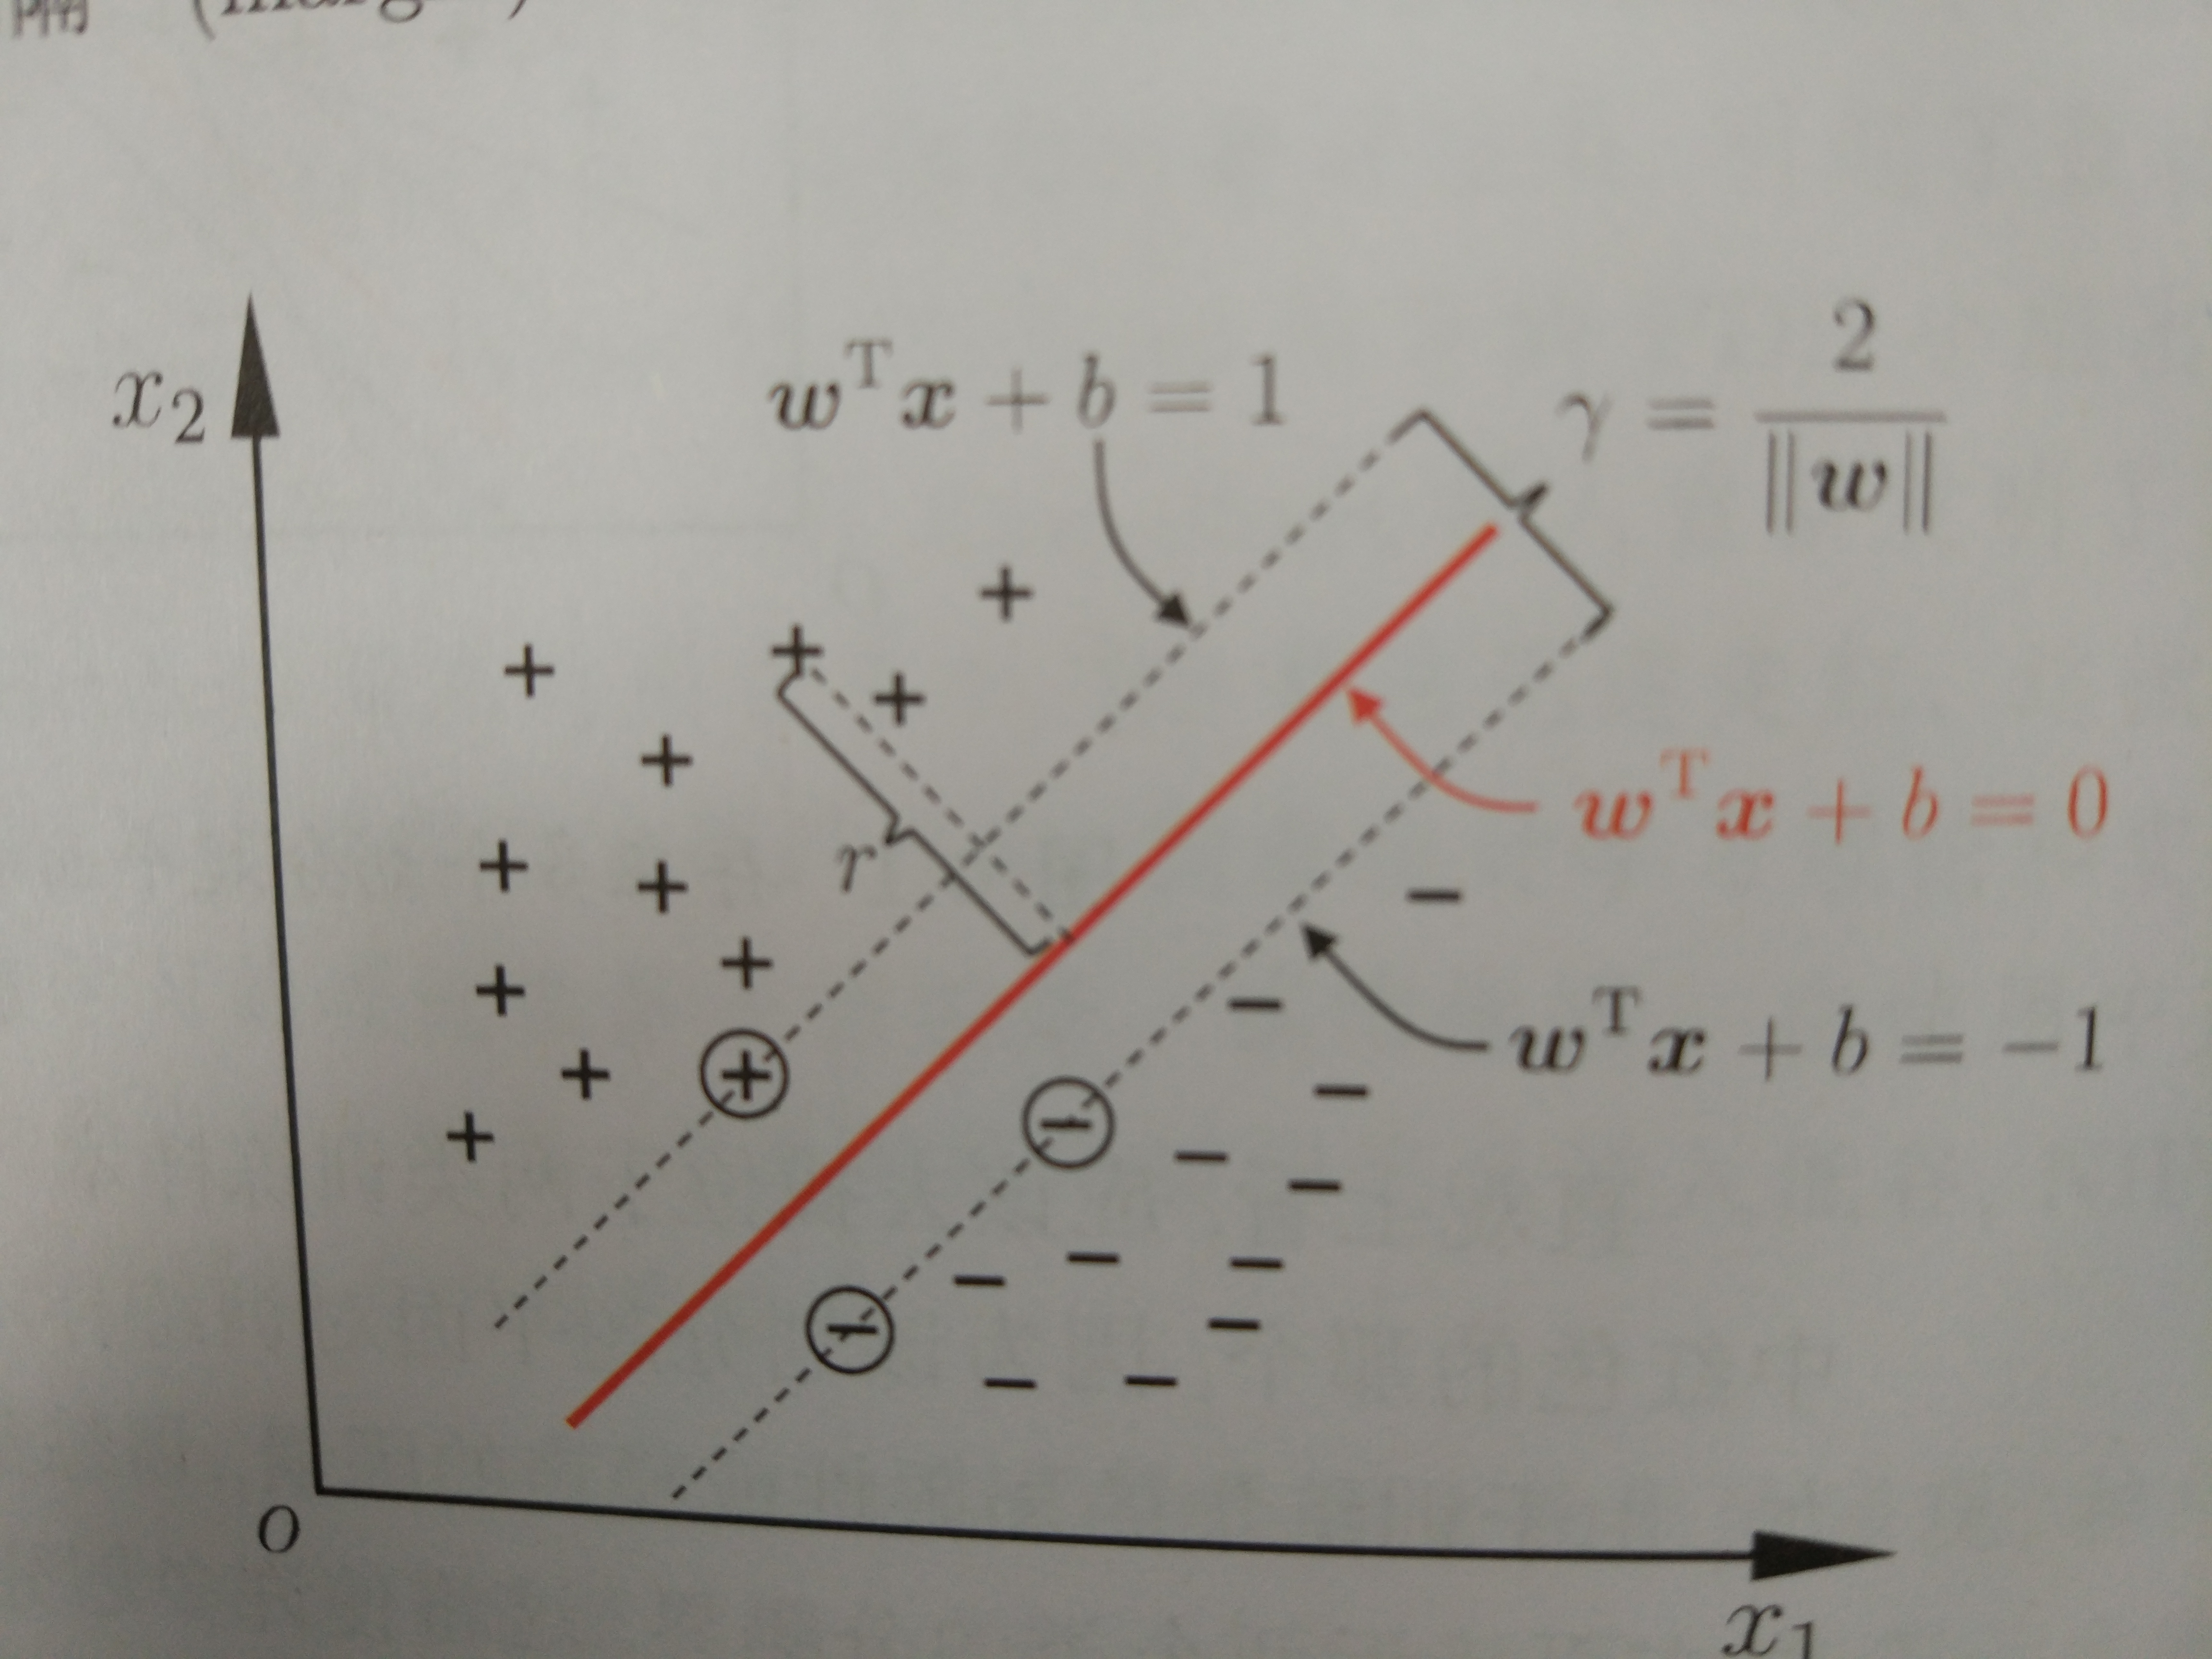
\includegraphics[width=5in]{6-2.jpg}
\caption{支持向量与间隔}
\label{6-2}
\end{figure}

欲找到具有``最大间隔"(maximum margin)的划分超平面,即



\begin{equation}
\begin{split}        %换行 
 {\underset{\boldsymbol{\omega},b}{max}} \quad \frac{2}{\parallel \boldsymbol{\omega} \parallel}  \\
 s.t. \quad y_{i}(\boldsymbol{\omega}^{T}\boldsymbol{x}_{i}+b) \geqslant 1, \quad i= 1,2, \ldots ,m.
\end{split}
\label{6-5}
\end{equation}

$b$通过约束隐式地影响$\boldsymbol{\omega}$,所以间隔与$b$和$\boldsymbol{\omega}$都有关.

式\ref{6-5}可以重写为:

\begin{equation}
\begin{split}        %换行 
 {\underset{\boldsymbol{\omega},b}{max}} \quad \frac{\parallel \boldsymbol{\omega} \parallel^{2}}{2} \\
 s.t. \quad y_{i}(\boldsymbol{\omega}^{T}\boldsymbol{x}_{i}+b) \geqslant 1, \quad i= 1,2, \ldots ,m.
\end{split}
\label{6-6}
\end{equation}

\subsection{对偶问题}





%==========================================================================
\end{document}
